\documentclass[12pt]{article}
\usepackage[UTF8]{ctex}
\usepackage{geometry}
\usepackage{listings}
\usepackage{graphicx}
\usepackage{subfigure}
\usepackage{array}
\usepackage{caption}    
\usepackage{float}
\usepackage{subfloat}
\usepackage{hyperref}
\usepackage{bookmark}
\usepackage{amsmath}
\usepackage{url}

\geometry{left=15mm,right=15mm,top=20mm,bottom=20mm}
\title{第六次作业报告}
\author{PB21010362 汪兆辰}
\date{\today}
\newcommand{\upcite}[1]{\textsuperscript{\textsuperscript{\cite{#1}}}}

\begin{document}

\maketitle

\section{算法介绍}
为了在网格变形的过程中能够保持局部细节和结构,论文\upcite{1}引入了laplace坐标来进行网格编辑. 不同与传统的坐标采用网格顶点的绝对位置,laplace坐标考虑网格顶点间的相对位置.
对网格上每个点定义laplace坐标:
\begin{equation}
    \delta _i=\mathcal{L} (v_i)
\end{equation}
其中$\mathcal{L} (v_i)$是关于顶点$v_i$及其邻接点的函数,根据权重选取的不同有不同的形式. 使用均匀权重时,laplace坐标表示为:
\begin{equation}
    \mathcal{L} (v_i)=v_i-\frac{1}{d_i} \sum_{j \in \mathcal{N} _i} v_j
\end{equation}
选用cot权重时,laplace坐标表示为:
\begin{equation}
    \mathcal{L} (v_i)=v_i-\sum_{j \in \mathcal{N}_i} \frac{\cot \alpha _j +\cot \beta _j}{2}
\end{equation}
其中$\mathcal{N}_i$为与$v_i$邻接的点的集合,$d_i=|\mathcal{N}_i|$,$\alpha_j,\beta_j$为$v_i v_j$所对的两个角.

得到所有点的laplace坐标$\Delta=LV$后,可以在$\Delta$上对顶点进行操作,但由于rank(L)=n-1, 无法直接还原顶点坐标V,于是考虑固定部分控制点,并定义能量:
\begin{equation}
    E(V')=\sum_{i=1}^{n} \left\lVert \delta_i -\mathcal{L}(v_i')\right\rVert ^2+\sum_{i=m}^{n}\left\lVert v_i'-u_i\right\rVert ^2  
\end{equation}
只需求解$E(V')$的最小值,即可得到经过操作后的网格. 这可以转化为求解以下方程的最小二乘解:
\begin{equation}
    \begin{pmatrix}
        L\\
        c
    \end{pmatrix}
    V=
    \begin{pmatrix}
        \Delta \\
        c'
    \end{pmatrix}
\end{equation}
其中L,V定义如前文所述,c为控制点的位置,$c'$为控制点的坐标.

\section{算法实现}
算法的实现部分用c++建立了laplace算子矩阵L,并将计算得到的L及其他需要的数据传入matlab,利用matlab脚本计算方程(5)的最小二乘解.

\subsection{网格变形}
利用均匀权重的Laplace算子可以通过网格的邻接矩阵经过矩阵运算得出:
\begin{equation}
    L=I-D^{-1}A
\end{equation}
其中A为网格的邻接矩阵,D是$d_i$构成的对角阵,容易从邻接矩阵直接计算出. 由于邻接矩阵是稀疏的,考虑采用Eigen库的SparseMatrix,利用三元组进行赋值. 
三元组的建立需要遍历读入网格时得到的顶点间的拓扑关系meshF,其中每一行为一个三角形面的三个顶点标号,对每个三角形面按顺时针、逆时针各遍历一遍,就得到了网格的邻接矩阵. 
D只需对A的每一行求和并化为对角阵即可,这样就得到了Laplace矩阵L.

方程(5)的建立比较平凡,因为控制点的坐标已经在P2PVtxIds中给出,只需取出对应的点填入矩阵方程对应位置即可. 令方程(5)为$Az=b$, z的最小二乘解可以由:
\begin{equation}
    A^T Az=A^T b
\end{equation}
给出,z的前n行即为编辑后的网格坐标. 

\subsection{利用cot权重}
采用cot权重对laplace算子赋值选择了直接对空的稀疏矩阵对应位置赋值. 对每个三角形面,可以得到每条边对应的两个角的其中一个,因而考虑对建立的Cot\_Mat的每个位置赋两次值,这需要允许赋值的位置非空,因此利用coeffRef方法,例如:
\begin{lstlisting}
    Cot_Mat.coeffRef(temp(0,j),temp(0,(j+1)%3))+=Cot(...)/2;
\end{lstlisting}

注意到没有现有的函数可以直接根据三角形的三个顶点位置给出cot值,因而在函数中自定义lambda表达式:
\begin{lstlisting}
    auto Cot = [X](int i, int j,int k) {
        Eigen::Vector3f ki=X.row(i)-X.row(k);
        Eigen::Vector3f kj=X.row(j)-X.row(k);
        float cosVal = ki.dot(kj) / (ki.norm() * kj.norm());
        float angle = acos(cosVal);
        return 1/tanf(angle);
    };
\end{lstlisting}
该lambda表达式值捕获了函数中的顶点坐标X,输入参数i,j,k为三个顶点的标号,返回边ij所对的角的cot值. 

\subsection{实现效果}

\begin{figure}[htbp]
    \centering
    \subfigure[uniform]{
        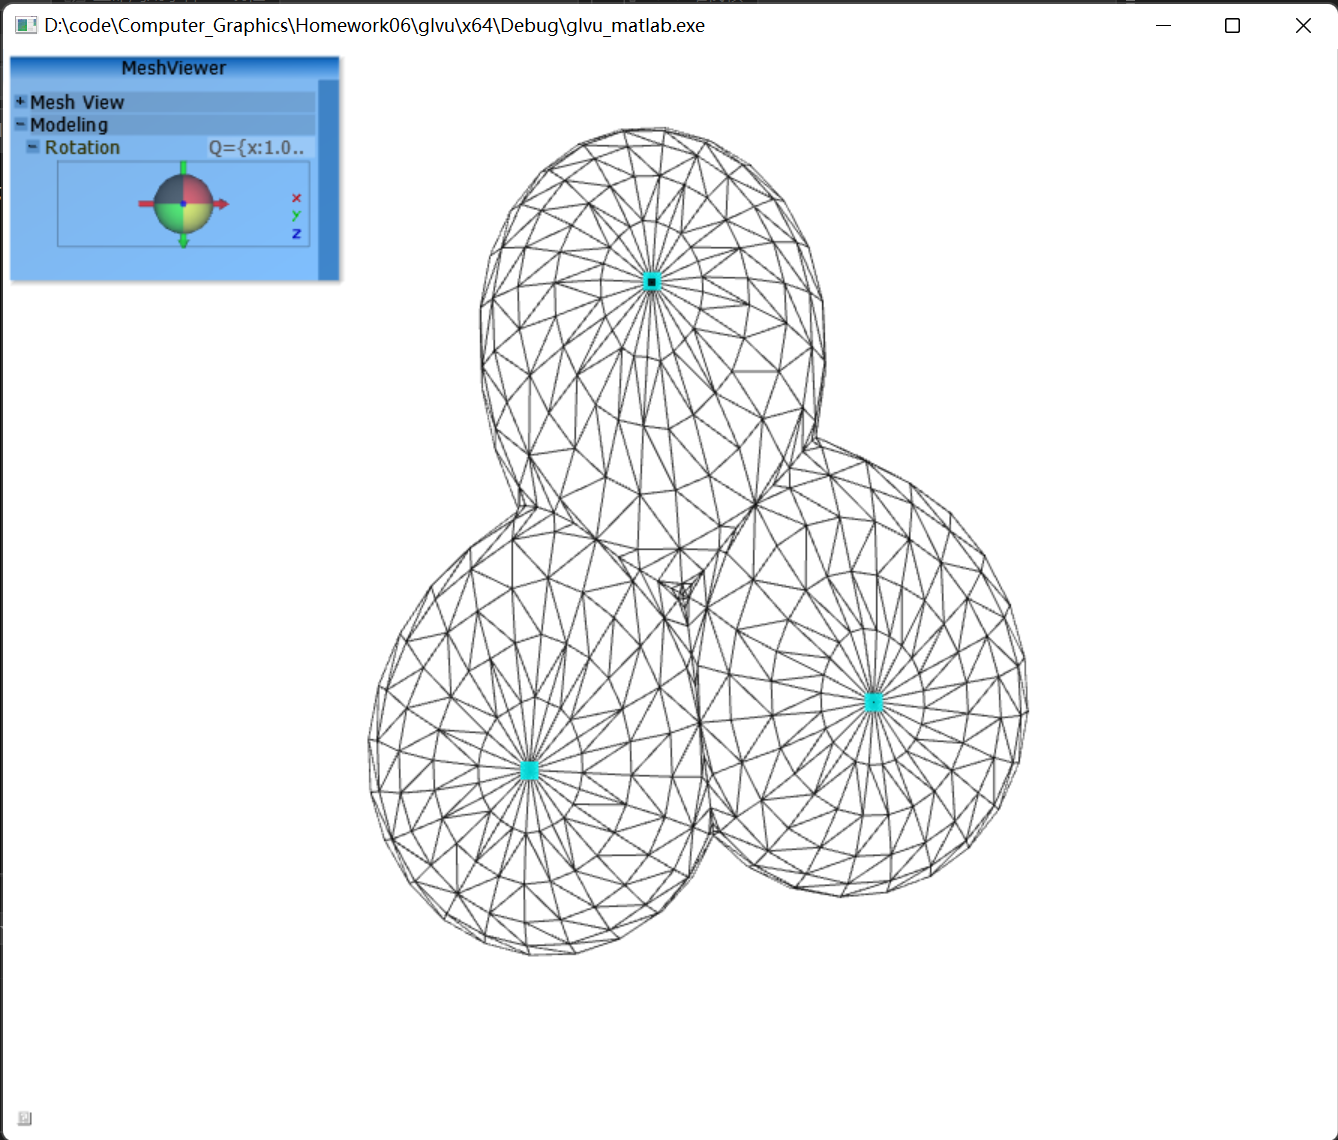
\includegraphics[width=0.45\textwidth]{pic1.png}
    }
    \subfigure[cot]{
        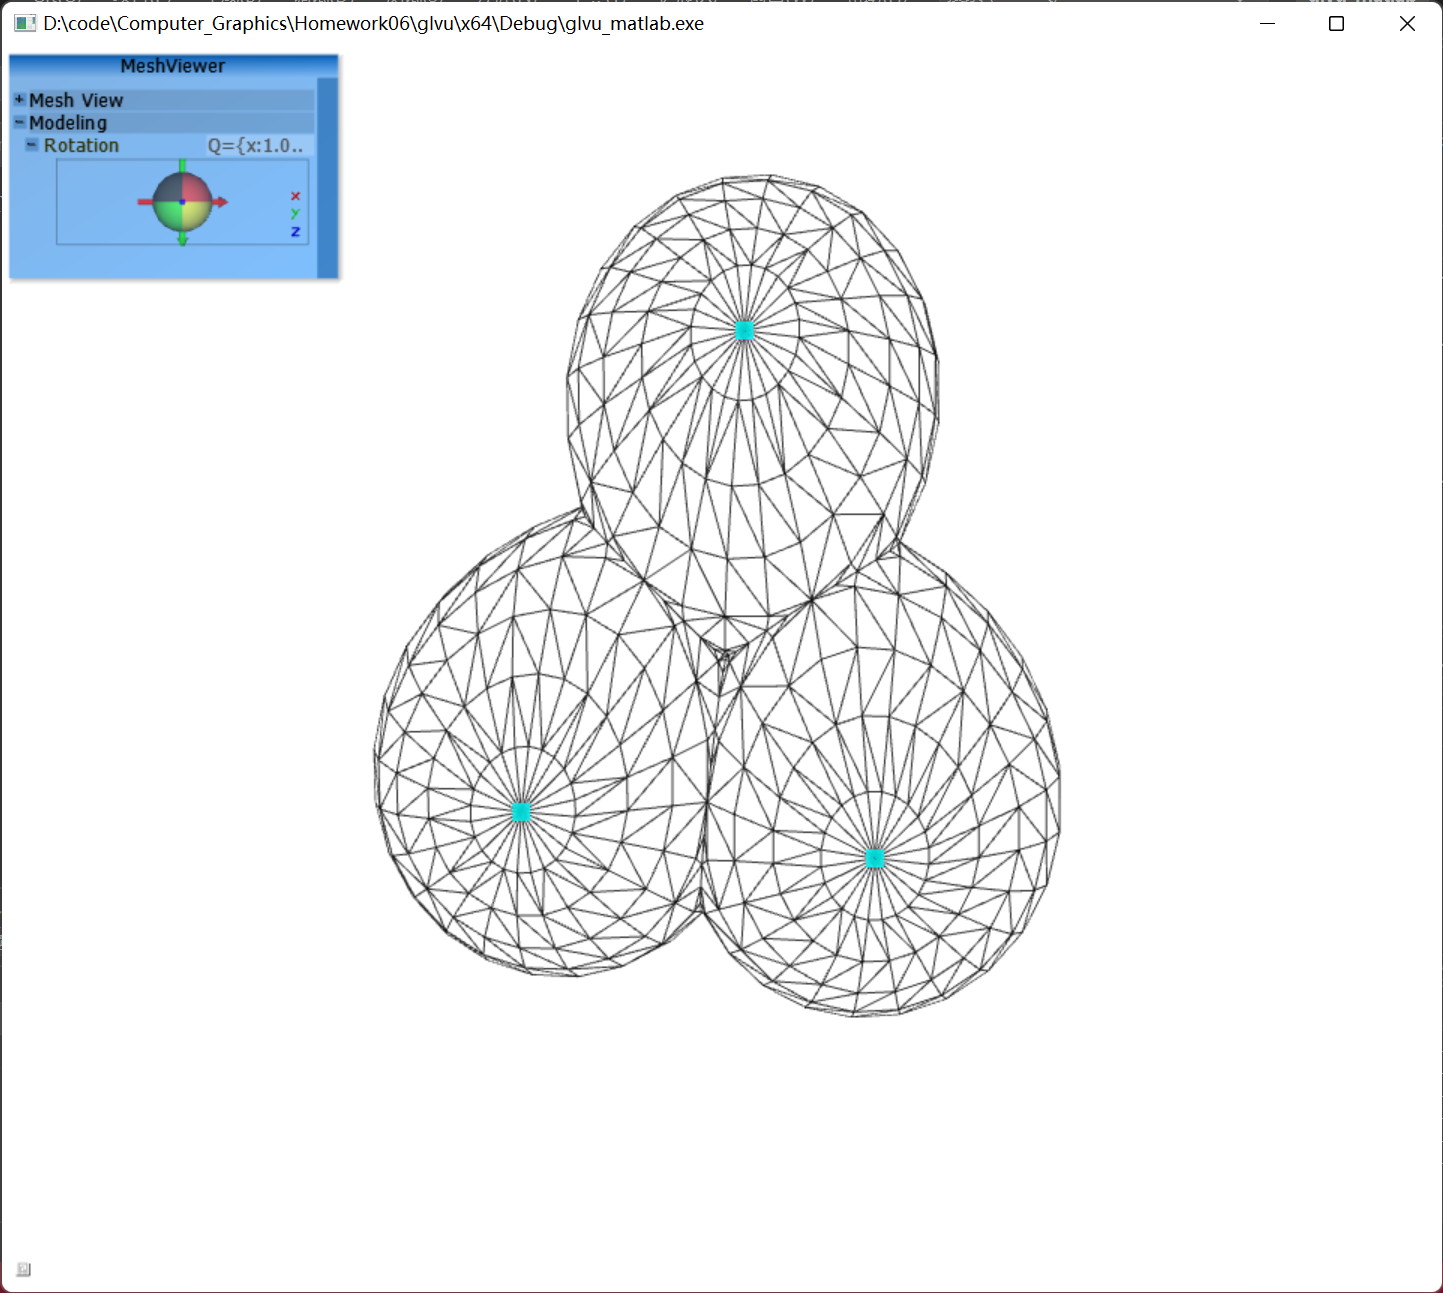
\includegraphics[width=0.45\textwidth]{pic2.png}
    }
\end{figure}

\section{bonus:laplace坐标下的旋转操作}

由于在laplace坐标下,旋转操作前后的局部细节无法很好的保持,于是仍然考虑对定义的能量找到最小二乘解,从而确定变换矩阵. 在这里定义了能量:
\begin{equation}
    E(V')=\sum_{i=1}^{n} \left\lVert T_i (V') \delta _i- \mathcal{L}(v_i ')\right\rVert ^2+\sum_{i=m}^{n}\left\lVert v_i '-u_i\right\rVert ^2 
\end{equation}
为了求解这一方程的最小二乘解,将其转化为类似于方程(5)的形式:
\begin{equation}
    \begin{pmatrix}
        L\\
        c
    \end{pmatrix}
    V=
    \begin{pmatrix}
        \Delta'\\
        c'
    \end{pmatrix}
\end{equation}
其中$\Delta'$为将控制点旋转后的laplace坐标.

在这里旋转是由用户操作返回的四元数组myRotation定义的,将其传入matlab并调用quat2dcm函数,从而得到对应的三维旋转矩阵,再将$\Delta$中控制点右乘该矩阵即可,其他求解过程相同.
为了能够实时生成旋转后的图像,需要用到回调函数实时对更新的myRotation调用方法,(由于没有看懂老师讲的TwAddVarCB里面setCallBack和getCallBack是什么东西)考虑使用GL中的glutTimeFunc来登记回调函数,其中回调函数定义如下: 
\begin{lstlisting}
void rotationcallback(int) {
    if (...) {\\myRotation has been updated
        for (int i = 0; i < 4; i++)recRotation[i] = myRotation[i];
        meshDeform();
    }
    glutTimerFunc(1, rotationcallback, 1);
}
\end{lstlisting}
其中利用recRotation来判断用户是否更新了myRotation.




\begin{thebibliography}{3}
    \bibitem{1} O. Sorkine et al. Laplacian Surface Editing. SGP 2004
    \bibitem{2} \url{https://cloud.tencent.com/developer/article/1745166}

\end{thebibliography}


\end{document}